\documentclass{standalone}
\usepackage{tikz}
\usetikzlibrary{patterns, positioning}

\begin{document}
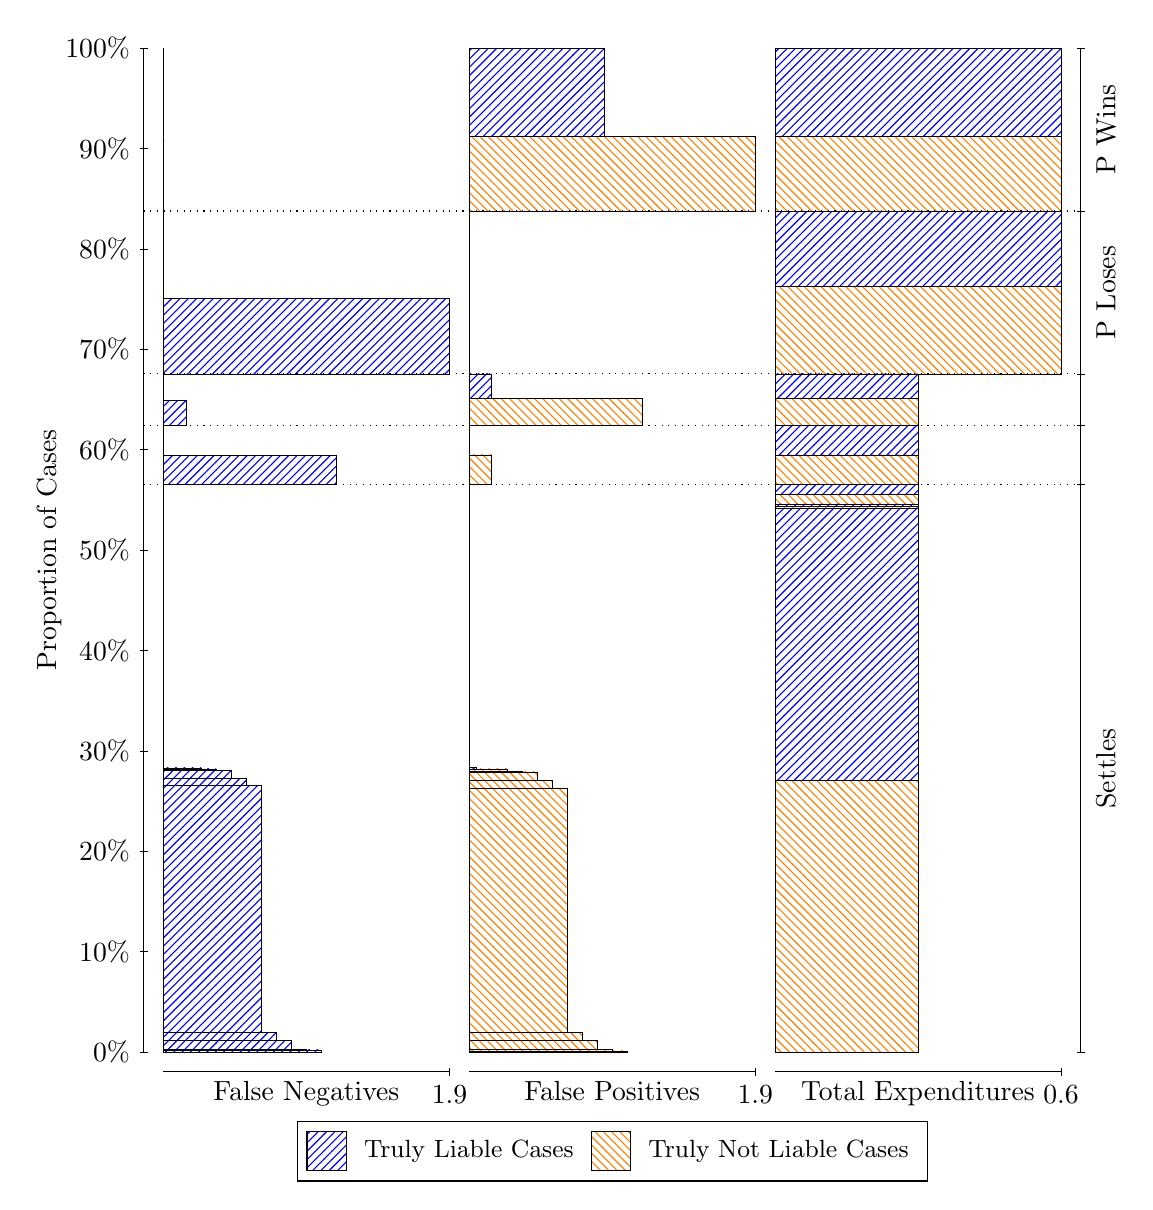
\begin{tikzpicture}
\draw[black, very thin] (1.5,1.75) -- (1.5,14.5);
\node[rotate=90, anchor=center] at (0.3, 8.125) {Proportion of Cases};
\draw[black, very thin] (1.45,1.75) -- (1.55,1.75);
\node[anchor=east] at (1.45, 1.75) {0\%};
\draw[black, very thin] (1.45,3.025) -- (1.55,3.025);
\node[anchor=east] at (1.45, 3.025) {10\%};
\draw[black, very thin] (1.45,4.3) -- (1.55,4.3);
\node[anchor=east] at (1.45, 4.3) {20\%};
\draw[black, very thin] (1.45,5.575) -- (1.55,5.575);
\node[anchor=east] at (1.45, 5.575) {30\%};
\draw[black, very thin] (1.45,6.85) -- (1.55,6.85);
\node[anchor=east] at (1.45, 6.85) {40\%};
\draw[black, very thin] (1.45,8.125) -- (1.55,8.125);
\node[anchor=east] at (1.45, 8.125) {50\%};
\draw[black, very thin] (1.45,9.4) -- (1.55,9.4);
\node[anchor=east] at (1.45, 9.4) {60\%};
\draw[black, very thin] (1.45,10.675) -- (1.55,10.675);
\node[anchor=east] at (1.45, 10.675) {70\%};
\draw[black, very thin] (1.45,11.95) -- (1.55,11.95);
\node[anchor=east] at (1.45, 11.95) {80\%};
\draw[black, very thin] (1.45,13.225) -- (1.55,13.225);
\node[anchor=east] at (1.45, 13.225) {90\%};
\draw[black, very thin] (1.45,14.5) -- (1.55,14.5);
\node[anchor=east] at (1.45, 14.5) {100\%};

\draw[black, very thin] (13.4,1.75) -- (13.4,14.5);
\draw[black, very thin] (13.35,1.75) -- (13.45,1.75);
\node[anchor=west] at (13.35, 1.75) {};
\draw[black, very thin] (13.35,8.9546) -- (13.45,8.9546);
\node[anchor=west] at (13.35, 8.9546) {};
\draw[black, very thin] (13.35,9.7062) -- (13.45,9.7062);
\node[anchor=west] at (13.35, 9.7062) {};
\draw[black, very thin] (13.35,10.362) -- (13.45,10.362);
\node[anchor=west] at (13.35, 10.362) {};
\draw[black, very thin] (13.35,12.43) -- (13.45,12.43);
\node[anchor=west] at (13.35, 12.43) {};
\draw[black, very thin] (13.35,14.5) -- (13.45,14.5);
\node[anchor=west] at (13.35, 14.5) {};

\draw[black, very thin, pattern color=blue, pattern=north east lines] (1.75,1.75) rectangle (3.7579,1.7776);
\draw[black, very thin, pattern color=blue, pattern=north east lines] (1.75,1.7776) rectangle (3.5667,1.7878);
\draw[black, very thin, pattern color=blue, pattern=north east lines] (1.75,1.7878) rectangle (3.3754,1.8968);
\draw[black, very thin, pattern color=blue, pattern=north east lines] (1.75,1.8968) rectangle (3.1842,1.9982);
\draw[black, very thin, pattern color=blue, pattern=north east lines] (1.75,1.9982) rectangle (2.993,5.1327);
\draw[black, very thin, pattern color=blue, pattern=north east lines] (1.75,5.1327) rectangle (2.8018,5.2236);
\draw[black, very thin, pattern color=blue, pattern=north east lines] (1.75,5.2236) rectangle (2.6105,5.3281);
\draw[black, very thin, pattern color=blue, pattern=north east lines] (1.75,5.3281) rectangle (2.4193,5.3449);
\draw[black, very thin, pattern color=blue, pattern=north east lines] (1.75,5.3449) rectangle (2.2281,5.359);
\draw[black, very thin, pattern color=orange, pattern=north west lines] (1.75,5.359) rectangle (1.75,8.9546);
\draw[black, very thin, pattern color=blue, pattern=north east lines] (1.75,8.9546) rectangle (3.9491,9.3275);
\draw[black, very thin, pattern color=orange, pattern=north west lines] (1.75,9.3275) rectangle (1.75,9.7062);
\draw[black, very thin, pattern color=blue, pattern=north east lines] (1.75,9.7062) rectangle (2.0368,10.022);
\draw[black, very thin, pattern color=orange, pattern=north west lines] (1.75,10.022) rectangle (1.75,10.362);
\draw[black, very thin, pattern color=blue, pattern=north east lines] (1.75,10.362) rectangle (5.3833,11.316);
\draw[black, very thin, pattern color=orange, pattern=north west lines] (1.75,11.316) rectangle (1.75,12.43);
\draw[black, very thin, pattern color=orange, pattern=north west lines] (1.75,12.43) rectangle (1.75,13.376);
\draw[black, very thin, pattern color=blue, pattern=north east lines] (1.75,13.376) rectangle (1.75,14.5);
\draw[black, very thin, pattern color=orange, pattern=north west lines] (5.6333,1.75) rectangle (7.6412,1.7643);
\draw[black, very thin, pattern color=orange, pattern=north west lines] (5.6333,1.7643) rectangle (7.45,1.7829);
\draw[black, very thin, pattern color=orange, pattern=north west lines] (5.6333,1.7829) rectangle (7.2588,1.8968);
\draw[black, very thin, pattern color=orange, pattern=north west lines] (5.6333,1.8968) rectangle (7.0675,1.9959);
\draw[black, very thin, pattern color=orange, pattern=north west lines] (5.6333,1.9959) rectangle (6.8763,5.0961);
\draw[black, very thin, pattern color=orange, pattern=north west lines] (5.6333,5.0961) rectangle (6.6851,5.1943);
\draw[black, very thin, pattern color=orange, pattern=north west lines] (5.6333,5.1943) rectangle (6.6851,5.1974);
\draw[black, very thin, pattern color=orange, pattern=north west lines] (5.6333,5.1974) rectangle (6.4939,5.3062);
\draw[black, very thin, pattern color=orange, pattern=north west lines] (5.6333,5.3062) rectangle (6.3026,5.3167);
\draw[black, very thin, pattern color=orange, pattern=north west lines] (5.6333,5.3167) rectangle (6.1114,5.3456);
\draw[black, very thin, pattern color=blue, pattern=north east lines] (5.6333,5.3456) rectangle (5.7289,5.3597);
\draw[black, very thin, pattern color=blue, pattern=north east lines] (5.6333,5.3597) rectangle (5.6333,8.9546);
\draw[black, very thin, pattern color=orange, pattern=north west lines] (5.6333,8.9546) rectangle (5.9202,9.3333);
\draw[black, very thin, pattern color=blue, pattern=north east lines] (5.6333,9.3333) rectangle (5.6333,9.7062);
\draw[black, very thin, pattern color=orange, pattern=north west lines] (5.6333,9.7062) rectangle (7.8325,10.046);
\draw[black, very thin, pattern color=blue, pattern=north east lines] (5.6333,10.046) rectangle (5.9202,10.362);
\draw[black, very thin, pattern color=orange, pattern=north west lines] (5.6333,10.362) rectangle (5.6333,11.476);
\draw[black, very thin, pattern color=blue, pattern=north east lines] (5.6333,11.476) rectangle (5.6333,12.43);
\draw[black, very thin, pattern color=orange, pattern=north west lines] (5.6333,12.43) rectangle (9.2667,13.376);
\draw[black, very thin, pattern color=blue, pattern=north east lines] (5.6333,13.376) rectangle (7.3544,14.5);
\draw[black, very thin, pattern color=orange, pattern=north west lines] (9.5167,1.75) rectangle (11.333,5.1943);
\draw[black, very thin, pattern color=blue, pattern=north east lines] (9.5167,5.1943) rectangle (11.333,8.6538);
\draw[black, very thin, pattern color=orange, pattern=north west lines] (9.5167,8.6538) rectangle (11.333,8.6828);
\draw[black, very thin, pattern color=blue, pattern=north east lines] (9.5167,8.6828) rectangle (11.333,8.7104);
\draw[black, very thin, pattern color=orange, pattern=north west lines] (9.5167,8.7104) rectangle (11.333,8.8327);
\draw[black, very thin, pattern color=blue, pattern=north east lines] (9.5167,8.8327) rectangle (11.333,8.9546);
\draw[black, very thin, pattern color=orange, pattern=north west lines] (9.5167,8.9546) rectangle (11.333,9.3333);
\draw[black, very thin, pattern color=blue, pattern=north east lines] (9.5167,9.3333) rectangle (11.333,9.7062);
\draw[black, very thin, pattern color=orange, pattern=north west lines] (9.5167,9.7062) rectangle (11.333,10.046);
\draw[black, very thin, pattern color=blue, pattern=north east lines] (9.5167,10.046) rectangle (11.333,10.362);
\draw[black, very thin, pattern color=orange, pattern=north west lines] (9.5167,10.362) rectangle (13.15,11.476);
\draw[black, very thin, pattern color=blue, pattern=north east lines] (9.5167,11.476) rectangle (13.15,12.43);
\draw[black, very thin, pattern color=orange, pattern=north west lines] (9.5167,12.43) rectangle (13.15,13.376);
\draw[black, very thin, pattern color=blue, pattern=north east lines] (9.5167,13.376) rectangle (13.15,14.5);
\draw[black, dotted] (1.5,8.9546) -- (13.4,8.9546);
\draw[black, dotted] (1.5,9.7062) -- (13.4,9.7062);
\draw[black, dotted] (1.5,10.362) -- (13.4,10.362);
\draw[black, dotted] (1.5,12.43) -- (13.4,12.43);
\draw[black, very thin] (1.75,1.5) -- (5.3833,1.5);
\node[anchor=north] at (3.5667, 1.5) {False Negatives};
\draw[black, very thin] (5.3833,1.45) -- (5.3833,1.55);
\node[anchor=north] at (5.3833, 1.45) {1.9};

\draw[black, very thin] (5.6333,1.5) -- (9.2667,1.5);
\node[anchor=north] at (7.45, 1.5) {False Positives};
\draw[black, very thin] (9.2667,1.45) -- (9.2667,1.55);
\node[anchor=north] at (9.2667, 1.45) {1.9};

\draw[black, very thin] (9.5167,1.5) -- (13.15,1.5);
\node[anchor=north] at (11.333, 1.5) {Total Expenditures};
\draw[black, very thin] (13.15,1.45) -- (13.15,1.55);
\node[anchor=north] at (13.15, 1.45) {0.6};

\node[black, centered, rotate=90] at (13.72, 5.3523) {Settles};


\node[black, centered, rotate=90] at (13.72, 11.396) {P Loses};
\node[black, centered, rotate=90] at (13.72, 13.465) {P Wins};

\draw (7.449999999999999,1.5) node[draw=none] (baseCoordinate) {};
\begin{scope}[align=center]
        \matrix[scale=0.5, draw=black, below=0.5cm of baseCoordinate, nodes={draw}, column sep=0.1cm]{
            \node[rectangle, draw, minimum width=0.5cm, minimum height=0.5cm, pattern=north east lines, pattern color=blue] {}; &
            \node[draw=none, font=\small] (B) {Truly Liable Cases}; &
            \node[rectangle, draw, minimum width=0.5cm, minimum height=0.5cm, pattern=north west lines, pattern color=orange] {}; &
            \node[draw=none, font=\small] (B) {Truly Not Liable Cases}; \\
            };
\end{scope}

\end{tikzpicture}
\end{document}